%!TEX root = ../report.tex
\chapter{Implementation}\label{ch:implementation}

% TODO @all add introduction to implementation
\lipsum[2-4]

\section{Libraries}
% TODO @all add introduction to libraries
% -> why libraries?
% -> advantages?
% -> disadvantages?

\section{Frontend}

\subsection{Services}

\subsubsection{API Service}
% TODO @joernneumeyer & @mauritsvanderzee

\subsubsection{Auth Service}
% TODO @joernneumeyer & @mauritsvanderzee

\subsubsection{Contact Service}
% TODO @joernneumeyer & @mauritsvanderzee

\subsubsection{Debug Service?}
% TODO @joernneumeyer & @mauritsvanderzee
% @joernneumeyer shall we include debug service?

\subsubsection{Crypto Storage Service}
% TODO @joernneumeyer & @mauritsvanderzee

\subsubsection{Key Registry Service}
% TODO @joernneumeyer & @mauritsvanderzee

\subsubsection{Titp Service}
% TODO @joernneumeyer & @mauritsvanderzee

\subsubsection{Util Service}
% TODO @mauritsvanderzee

\subsection{Components}

\section{Backend}

\subsection{Database Connections}

\subsection{Services}

\subsubsection{Authentication Service}
% TODO @joernneumeyer

\subsubsection{File Service}
% TODO @all shall we just briefly mention that this might be a service for future features / development

\subsubsection{Identity Service}
% TODO @joernneumeyer

\subsubsection{Settings Service}
% TODO @maltecastner & tobiasjansen

\subsubsection{Reporting Service}
% TODO @maltecastner & tobiasjansen

The Settings service provides an interface to the admin panel frontend and carries out the settings to the other services
As visible from the [Use Case diagram](#Use case diagram) the Settings service carries out a few tasks by itself whilst forwarding certain other request to the [identity service](identity-service.md) and the [reporting service](reporting.md).
The use cases and their descriptions can be found on in the online documentation.

Use Case Diagram
%todo insert use case diagram
\begin{figure}[!ht]
    \centering
    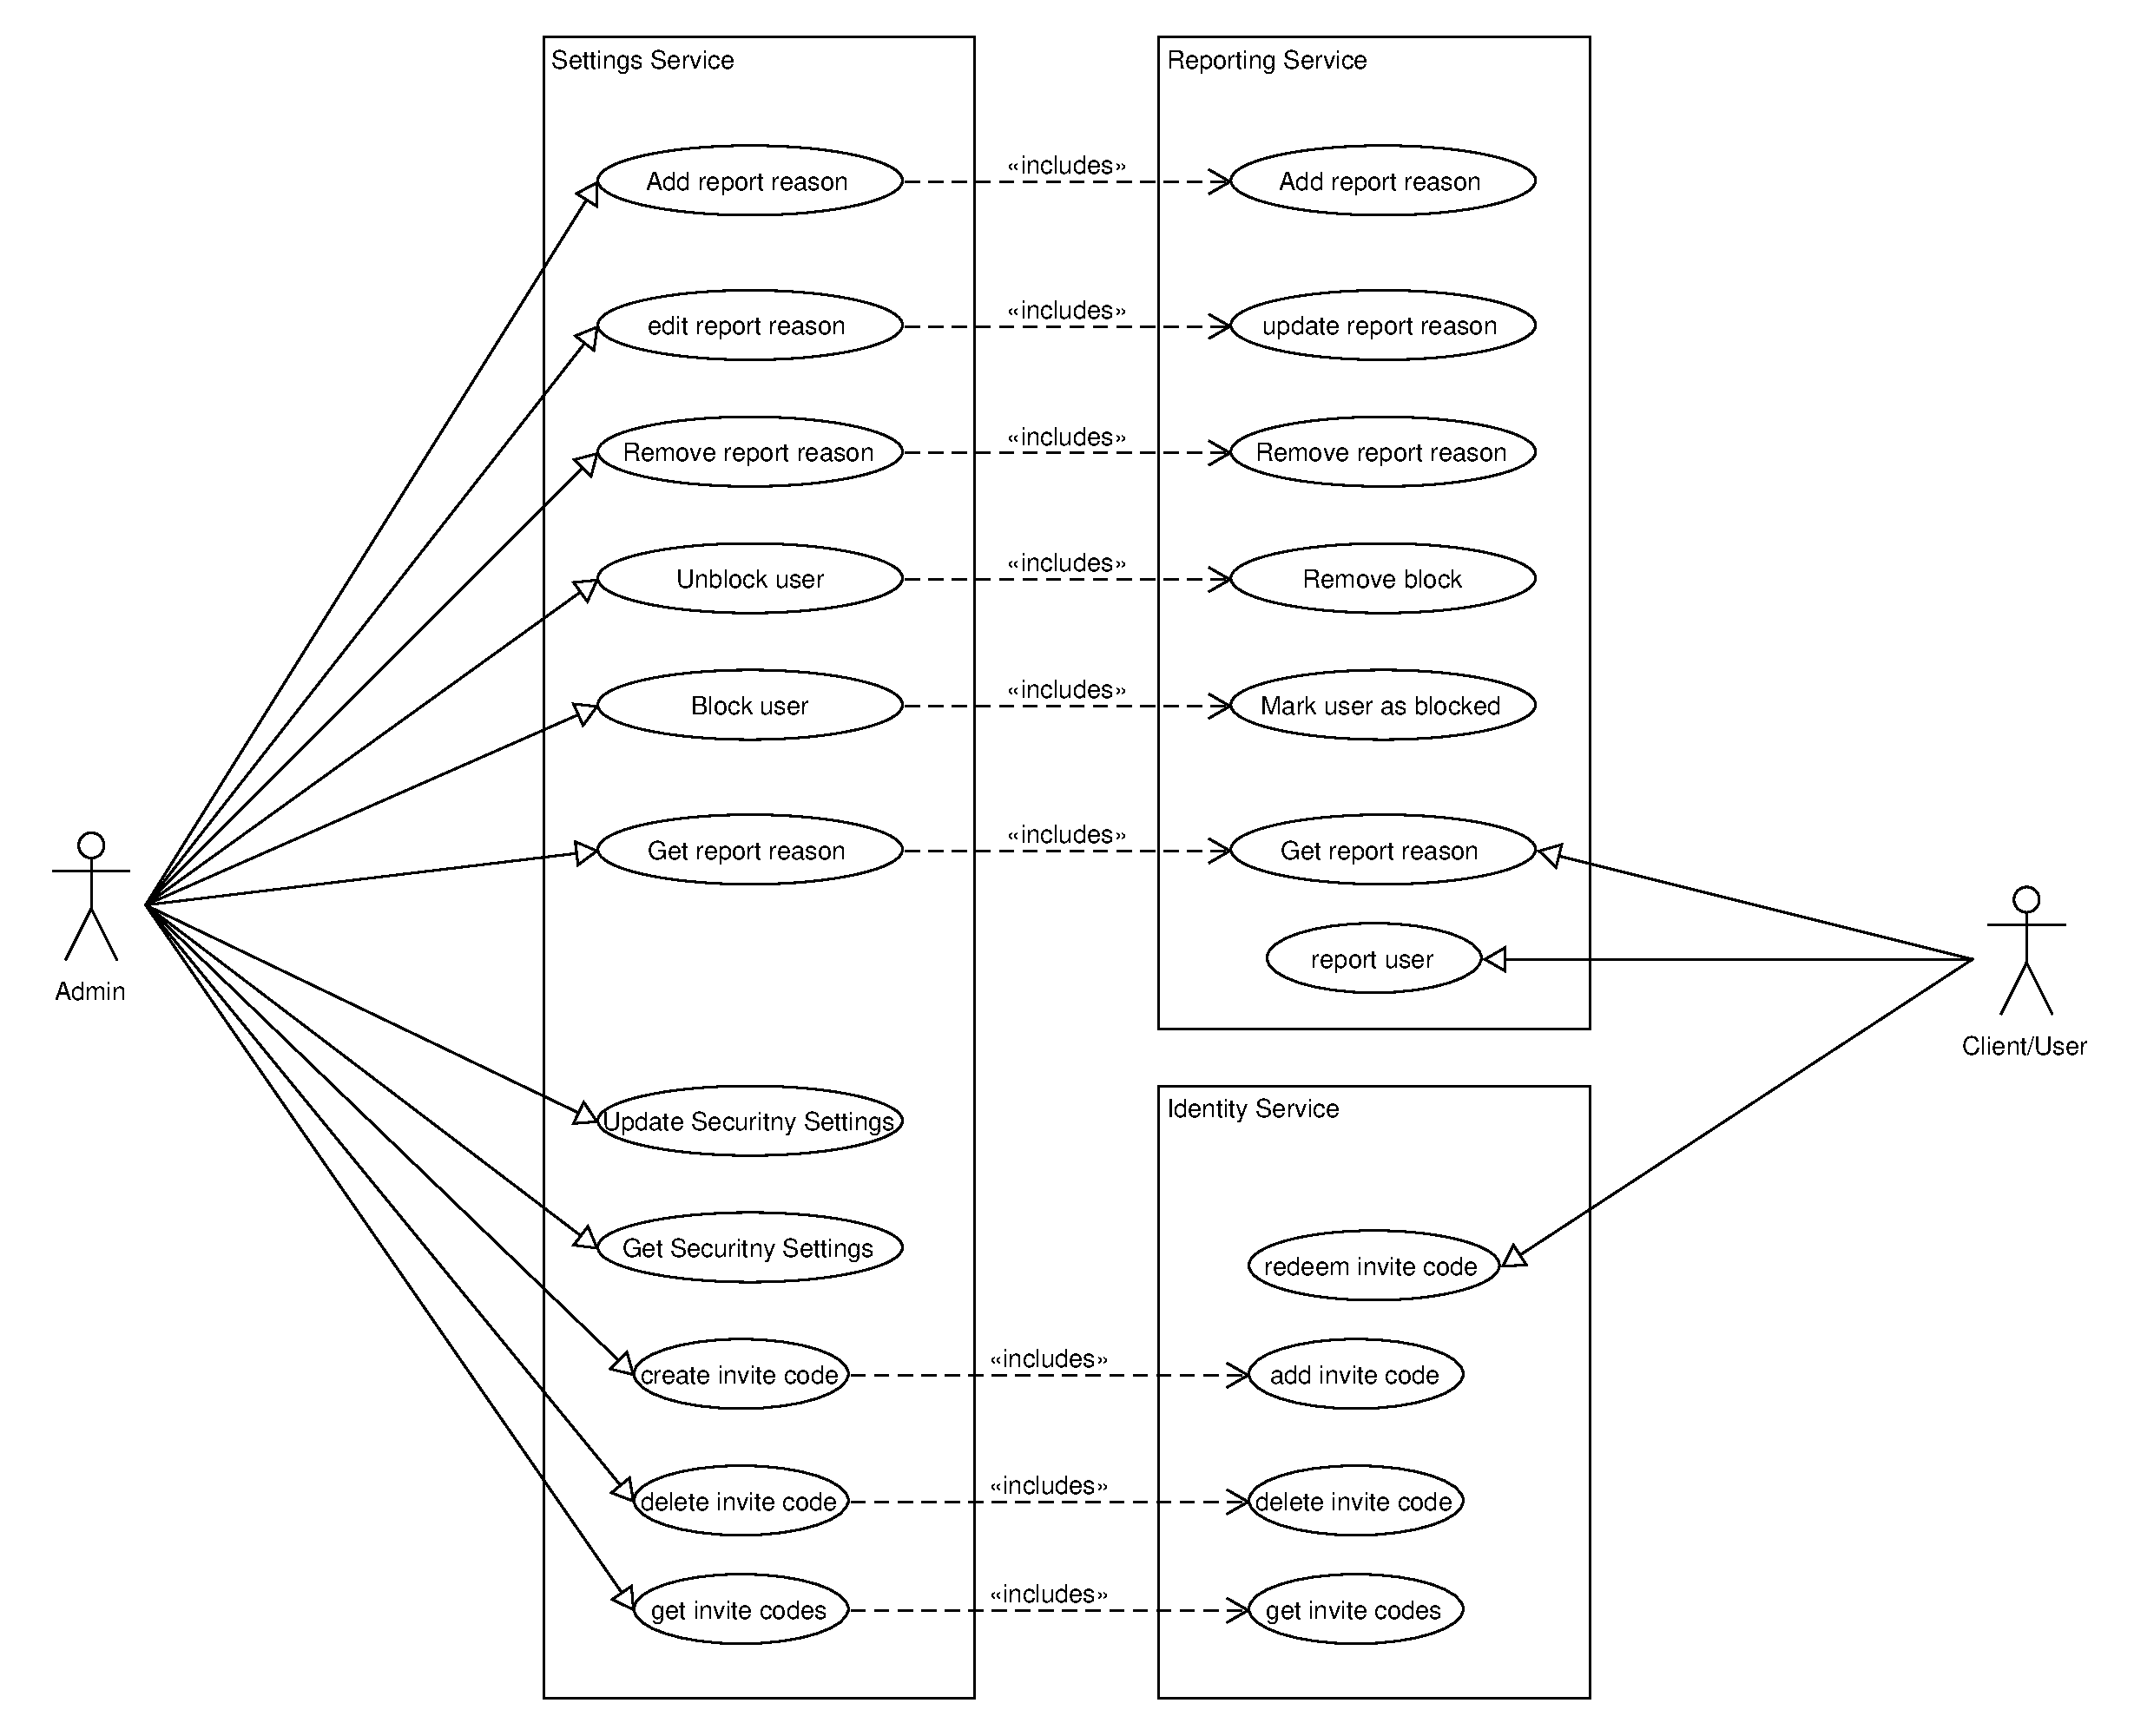
\includegraphics[width=1.0\textwidth]{./images/UseCaseDiagramAdminPanel.pdf}
    \caption{Use case diagram of the admin panel showing responsibility of each AP service~\ref{tab:usecasediagram}}
    \label{fig:ucd}
\end{figure}
![UseCaseDiagram](../../usecases/UseCaseDiagramAdminPanel.png)

###Rest interfaces
The settings service provides the following rest endpoints:
####Reporting settings
\begin{verbatim}

GET: /settings/report-reason
\end{verbatim}
Returns all report reasons as a JSON array.

\begin{verbatim}
POST: /settings/report-reason
body:
{
"reason": "some reason",
"max_report_violations": 5
}
\end{verbatim}
adds a new report reason.

\begin{verbatim}
PUT: /settings/report-reason
body:
{
"id": 123,
"reason": "some reason",
"max_report_violations": 5
}
\end{verbatim}
Edits an existing report reason.


\begin{verbatim}
DELETE: /settings/report-reason
headers:
- "id": 123
\end{verbatim}

Deletes a report reason with an id that is provided as a header.

####Security settings
\begin{verbatim}
GET: /settings/security
\end{verbatim}

returns the current security settings.

\begin{verbatim}
PUT: /settings/security
body:
{
"two_factor_auth": {
"on" : true,
"phone": false,
"email": true
},
"confirmed_emails_only": true,
"individual_pwd_req": {
"on": true,
"upper_case": true,
"number": true,
"special_char": true,
"reg_ex": false,
"reg_ex_string": "[]"
},
"inv_only": {
"on": false,
"inv_only_by_adm": false
}
}
\end{verbatim}
Edits the security settings. The new settings are provided in body.

##Example Add Report reason
![Sequence Diagram](SequenceDiagram_AddReportReason.svg)
The sequence diagram shows an example of the communication of the settings service with the aforementioned services.
Firstly by checking at the identity service, if the user who sent out the request is in fact an administrator and then adding the reason in the reporting service.
This way each service has a clearly defined task.

